\section{Das Analyseklassendiagramm}\label{Das AKD}
Aufgrund der Use-Case-Diagramme im Kapitel \ref{Use Case Diagramme} und der Wireframes im Kapitel \ref{Wireframes} wurde nun ein Klassendiagramm erstellt, welches die grundlegende Struktur der App verdeutlichen soll. Hierbei wurde bewusst auf Methoden und Klassenvariablen verzichtet um die \"Ubersichtlichkeit des Diagramms zu gew\"ahrleisten.

Im Klassendiagramm im Bild \ref{AKD} sind alle Klassen dargestellt, welche f�r die grundlegende Funktion der App notwendig sind. Hierbei wurde absichtlich auf das Einf�gen der Activity-Klassen verzichtet um die \"Ubersichtlichkeit zu gew�hrleisten.

Im mittleren Bereich des Diagramms sind die abstrakten Klassen "`Rule"', "`RuleCreator"', "`RuleObserver"' und die Klassen "`SMSRule"' und "`EMailRule"' zu finden. Mit diesen Klassen werden zum einen Regeln als Instanzen abgebildet, aber auch erstellt. Hierf\"ur wurde das Factory-Pattern in abge\"anderter Form verwendet. \cite{JavaPattern}

Im rechten Teil des Diagramms ist die abstrakte Oberklasse des Android \ac{SDK} BroadcastReceiver zu finden. Diese wird von den Klassen SMSReceiver und EMailReceiver erweitert, um das eingehen einer SMS oder E-Mail abzufangen.
\begin{figure}[!ht]
\centering
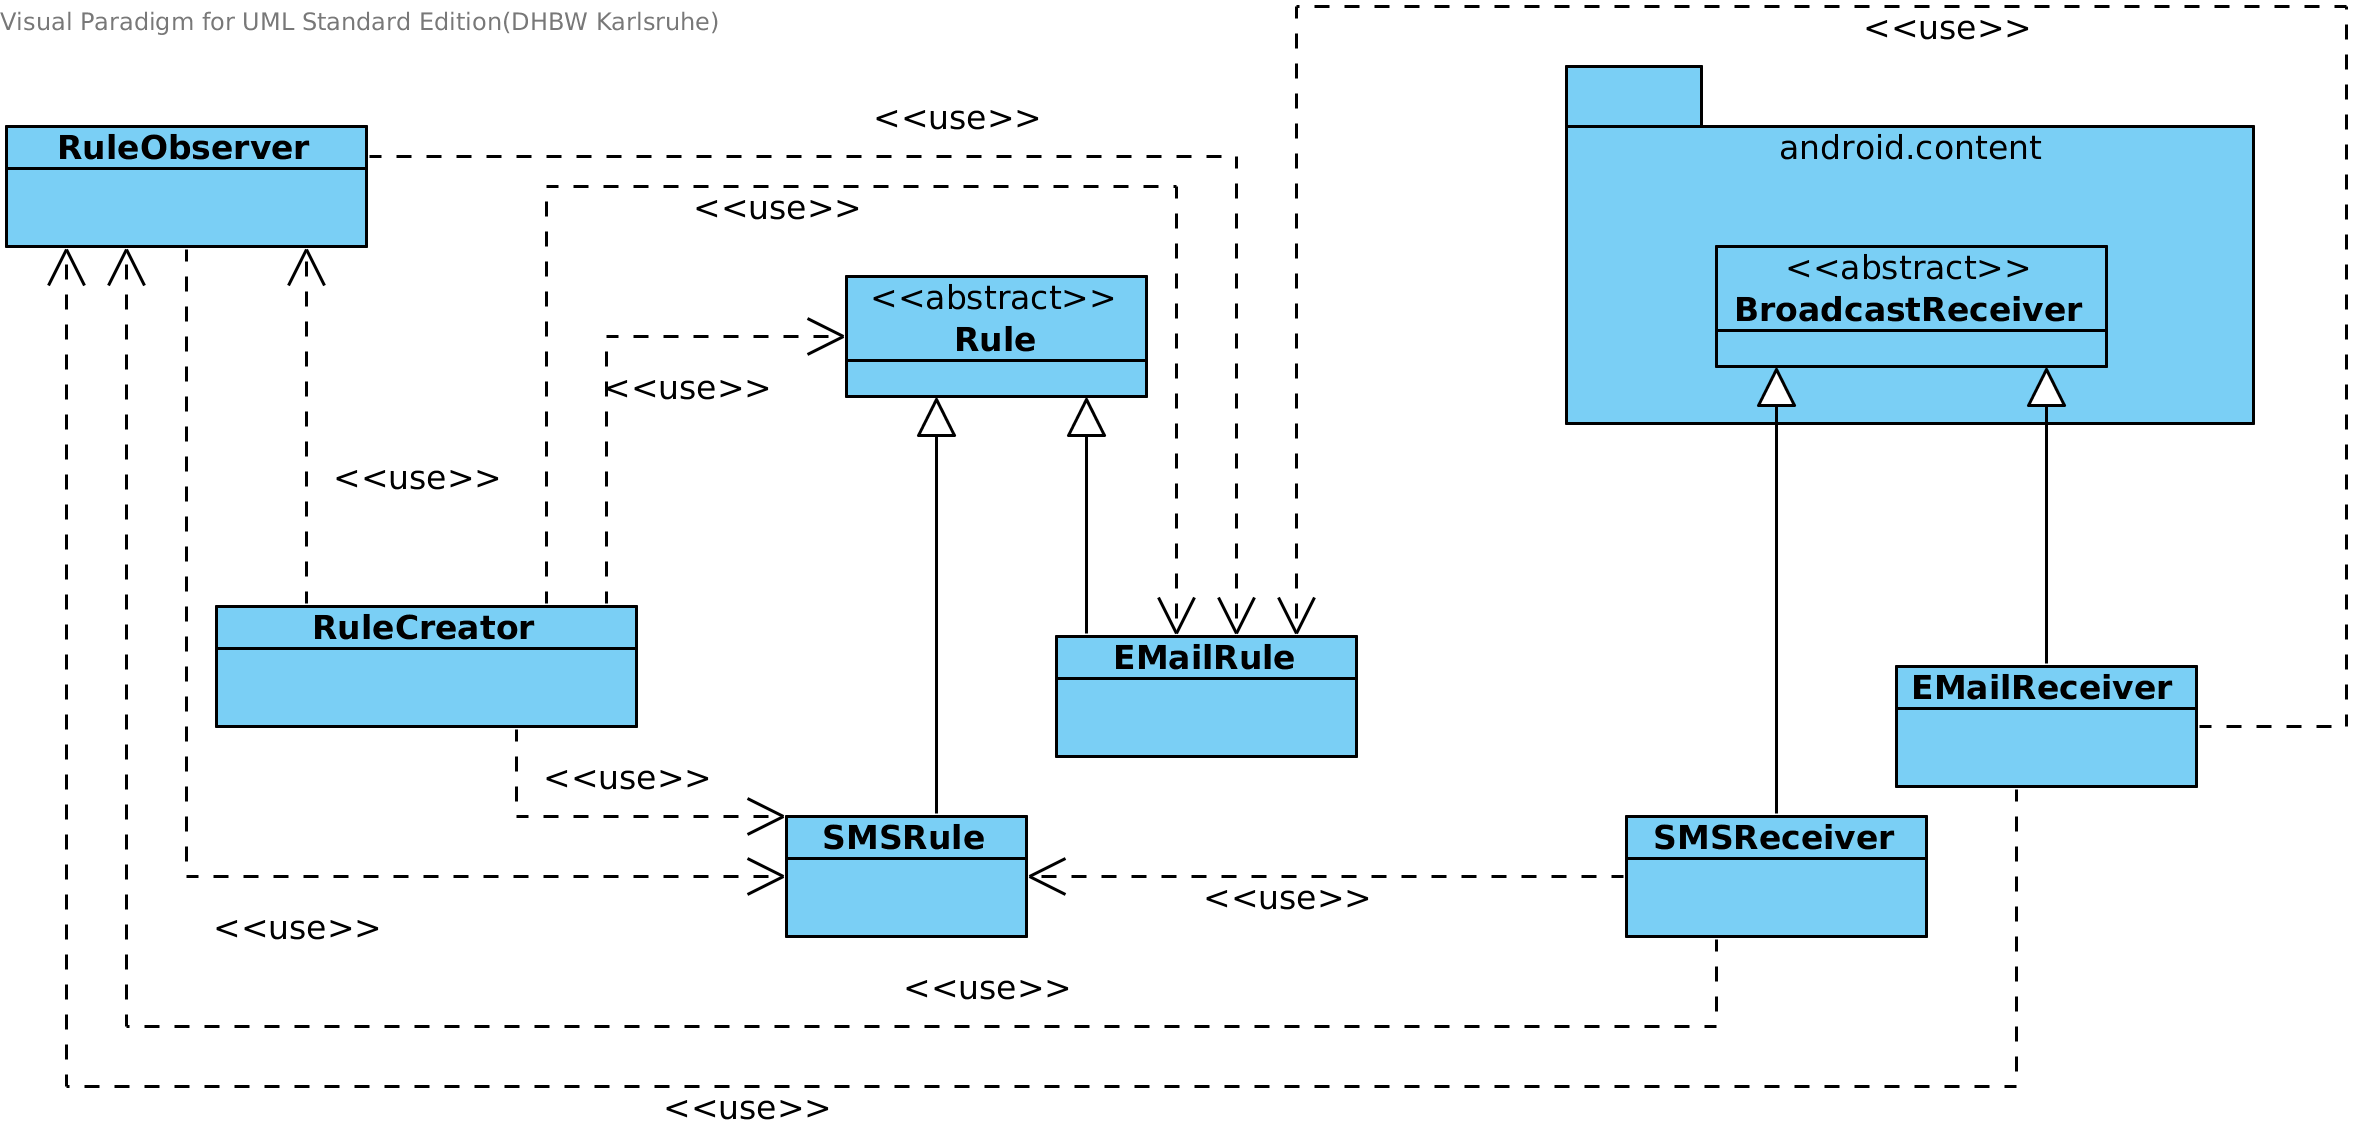
\includegraphics[width=16cm]{Bilder/AKD3.png}
\caption{Analyseklassendiagramm der App}
\label{AKD}
\centering
\end{figure}

\subsection{Das Factory Pattern} \label{AKD Factory Pattern}
Wie eben schon einmal erw\"ahnt, wurde das  Factory Pattern zwar verwendet, jedoch in einer abge\"anderten Version.
Dies war n\"otig, da eine Factory im Programm zu erst erstellt werden muss, bevor sie Verwendung finden kann. Da eine Android-App auf verschiedene Arten aufgerufen werden und gegebenenfalls andere Abl\"aufe stattfinden. So kann eine App zum Beispiel \"uber eine Activity gestartet werden oder \"uber einen BroadcastReceiver.

Zus\"atzlich m\"usste eine solche Factory bei einem Kontextwechsel mit \"ubergeben werden, wie es zum Beispiel der Fall w\"are, wenn eine neue Activity gestart wird. Denn unter Android haben einzelne Activity standardm\"a\ss{}ig keine Verbindung untereinander sondern werden wenn ben\"otigt aufgerufen.

Um nun nicht an jeder Stelle wo die Factory Verwendung findet zu pr\"ufen ob diese schon existiert und gegebenenfalls zu erstellen oder sie bei jedem Kontextwechsel zu \"ubergeben wurde sich aus rein praktischen Gr\"unden daf\"ur entschieden die Factory-Klasse (im Diagramm RuleCreator) nur mit statischen Methoden zu versehen.

Dies hat den Vorteil, das ihre Methoden an jeder Programmposition aufgerufen werden k\"onnen ohne eine Instanz der Klasse zu ben\"otigen.

Die Klasse RuleCreator kann alle Unterklassen der Klasse Rule erzeugen und ihre Werte ver\"andern. Dabei Folgen alle Methoden dem Schema:
\lstinputlisting{Code/FactorySchema.java}

\subsection{Das Observer Pattern} \label{AKD Observer Pattern}
\"Ahnlich wie beim Factory-Pattern ist auch die Problematik beim Observer-Pattern, hier kommt jedoch noch erschwerend hinzu, das der Nutzer und der Programmierer nur begrenzte Kontrolle dar\"uber haben wann eine App und ihre im Arbeitsspeicher befindlichen Daten geschlossen werden, dies \"ubernimmt Android automatisch.

Immer wenn Speicher ben\"otig wird, schlie\ss{}t Android im Hintergrund automatisch Apps, welche l\"anger nicht verwendet wurden sind.
Hier hat auch der Programmierer keine Chance dieses schlie\ss{}en zu verhindern.

Das Problem hierbei ist das alle im Arbeitsspeicher vorhandenen Daten verloren gehen, weswegen sie gespeichert werden w\"ussen.
Dieses speichern und laden von Regeln muss also der Observer \"ubernehmen. 

Die Klasse RuleObserver stellt den Observer dar, welcher das lesen und schreiben von wichtigen Regelinformationen auf das Filesystem \"ubernimmt.
Hierbei ist der Observer \"ahnlich wie die Factory aufgebaut, denn auch der Observer verf\"ugt nur \"uber statischen Methoden, welche das lesen und schreiben auf dem Filesystem \"ubernehmen.

Dies bietet wieder den Vorteil, dass ohne zuvor erstellte Instanz direkt auf die Methoden zugegriffen werden kann. Die Methoden serialisieren mit Hilfe der Jackson-Bibliotheke die Regeln zu JSON-Dokumenten und legen sie im Filesystem ab, beziehungsweise lesen die JSON-Dokumente und stellen mittels Deserialisierung wieder Java-Instanzen her.

\subsection{Das Model-View-Controller-Prinzip}
Unter dem Model-View-Controller-Prinzip wird ein Architekturmuster der Softwarearchitektur verstanden, welches ein Programm strukturiert.
Das Muster trennt klar die drei Aufgebenbereichen Modell, Pr\"asentation und Steuerung von einander.

Unter Modell, werden alle Klassen verstanden, welche Daten enthalten und welche Verarbeitet werden. Das Modell ist hierbei unabh\"angig und wird nur vom Controller bearbeitet, erstellt oder gel\"oscht. 

Die Pr\"asentation wird vom Controller gesteuert und stellt das Modell dar. Jegliche \"Anderung am View, wird durch den Controller auf das Model zur\"uck propagiert. Aus diesem Grund hat der View nicht die M\"oglichkeit eine \"Anderung am Model direkt vorzunehmen.

Dieses Verfahren bietet viele Vorteile, wie zum Beispiel die erh\"ohte Codeflexibilit\"at, was bedeutet, dass der Code entfolchten wird und so einzelne Module einfacher ausgetaucht oder ge\"andert werden k\"onnen. \cite{OOMVC} \cite{wikiMVC}

Unter Android bedeutet die Verwendung dieses Prinzips, dass die Activitys den View darstellen. Das Model wird \"uber Java-Klassen dargestellt, welche die Daten halten. Beim Controller jedoch ist es nicht ganz so einfach, da Android an dieser Stelle einige Aufgaben \"ubernimmt, wie die Speicherverwaltung oder das aufrufen des Views.

Trotzdem wurde im Projekt das MVC-Prinzip umgesetzt, wie sich zum einen im Klassendiagramm (im Bild \ref{AKD}) zeigt. Hier ist gut zu sehen, dass die einzelnen Klassen nur lose miteinander verbunden sind. Zum anderen ist zu sehen (Bild \ref{Projektstruktur in Eclipse}), dass die Projektstruktur in Eclipse eine \"ubersichtliche Struktur aufweist. So sind alle Klassen in ihren entsprechenden Packages untergebracht. Zus\"atzlich gibt es noch das Package "`util"', in welchem verschiedene Utillit-Klassen untergebracht sind.

\begin{figure}[!ht]
\centering
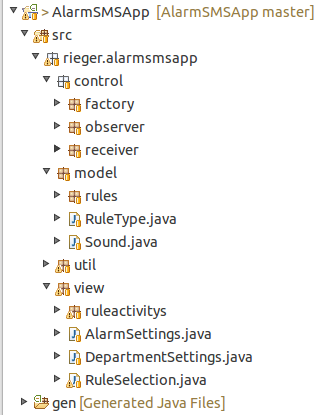
\includegraphics[width=6cm]{Bilder/ProjektStruktur.png}
\caption{Projektstruktur in Eclipse}
\label{Projektstruktur in Eclipse}
\centering
\end{figure}